%%%%%%%%%%%%%%%%%%%%%%%%%%%%%%%%%%%%%%%%%%%%%%%%%%%%%%%%%%%%%%%%%%%%%
% This is just an example/guide for you to refer to when submitting manuscripts to Frontiers, it is not mandatory to use Frontiers .cls files nor frontiers.tex

% This will only generate the Manuscript, the final article will be typeset by Frontiers after acceptance.   

% When submitting your files, remember to upload this *tex file, the pdf generated with it, the *bib file (if bibliography is not within the *tex) and all the figures.
%%%%%%%%%%%%%%%%%%%%%%%%%%%%%%%%%%%%%%%%%%%%%%%%%%%%%%%%%%%%%%%%%%%%%

%%% Version 3.4 Generated 2018/06/15 %%%
%%% You will need to have the following packages installed: datetime, fmtcount, etoolbox, fcprefix, which are normally inlcuded in WinEdt. %%%
%%% In http://www.ctan.org/ you can find the packages and how to install them, if necessary. %%%
%%%  NB logo1.jpg is required in the path in order to correctly compile front page header %%%

%\documentclass[utf8]{frontiersSCNS} % for Science, Engineering and Humanities and Social Sciences articles
\documentclass[utf8]{frontiersHLTH} % for Health articles
%\documentclass[utf8]{frontiersFPHY} % for Physics and Applied Mathematics and Statistics articles

%\setcitestyle{square} % for Physics and Applied Mathematics and Statistics articles
\usepackage{url,hyperref,lineno,microtype,subcaption}
\usepackage[onehalfspacing]{setspace}

\linenumbers


% Leave a blank line between paragraphs instead of using \\

%%% Please be aware that for original research articles we only permit a combined number of 15 figures and tables, one figure with multiple subfigures will count as only one figure.
%%% Use this if adding the figures directly in the mansucript, if so, please remember to also upload the files when submitting your article
%%% There is no need for adding the file termination, as long as you indicate where the file is saved. In the examples below the files (logo1.eps and logos.eps) are in the Frontiers LaTeX folder
%%% If using *.tif files convert them to .jpg or .png
%%%  NB logo1.eps is required in the path in order to correctly compile front page header %%%

%%% If you are submitting a figure with subfigures please combine these into one image file with part labels integrated.
%%% If you don't add the figures in the LaTeX files, please upload them when submitting the article.
%%% Frontiers will add the figures at the end of the provisional pdf automatically
%%% The use of LaTeX coding to draw Diagrams/Figures/Structures should be avoided. They should be external callouts including graphics.

%% Figures, tables, and images will be published under a Creative Commons CC-BY licence and permission must be obtained for use of copyrighted material from other sources (including re-published/adapted/modified/partial figures and images from the internet). It is the responsibility of the authors to acquire the licenses, to follow any citation instructions requested by third-party rights holders, and cover any supplementary charges.


\def\keyFont{\fontsize{8}{11}\helveticabold }
\def\firstAuthorLast{H. Kim {et~al.}} %use et al only if is more than 1 author
\def\Authors{Haedong Kim\,$^{1}$, Hui Yang\,$^{1,*}$, Andrew R. Ednie\,$^{2}$ and Eric S. Bennett\,$^{2}$}
% Affiliations should be keyed to the author's name with superscript numbers and be listed as follows: Laboratory, Institute, Department, Organization, City, State abbreviation (USA, Canada, Australia), and Country (without detailed address information such as city zip codes or street names).
% If one of the authors has a change of address, list the new address below the correspondence details using a superscript symbol and use the same symbol to indicate the author in the author list.
\def\Address{$^{1}$Complex Systems Monitoring, Modeling, and Control Laboratory, The Pennsylvania State University, University Park, PA, USA \\
$^{2}$Department of Neuroscience, Cell Biology and Physiology, Wright State University, Dayton, OH, USA}
% The Corresponding Author should be marked with an asterisk
% Provide the exact contact address (this time including street name and city zip code) and email of the corresponding author
\def\corrAuthor{310 Leonhard Building, University Park, PA 16802-4400, USA}
\def\corrEmail{huiyang@psu.edu}


\begin{document}
\onecolumn
\firstpage{1}

\title[Simulation-guided Data Assimilation of K\textsubscript{v}]{Simulation-guided Data Assimilation for Kinetics Modeling of Potassium Channel Isoforms in Mouse Cardiomyocytes} 

\author[\firstAuthorLast ]{\Authors} %This field will be automatically populated
\address{} %This field will be automatically populated
\correspondance{} %This field will be automatically populated

\extraAuth{}% If there are more than 1 corresponding author, comment this line and uncomment the next one.
%\extraAuth{corresponding Author2 \\ Laboratory X2, Institute X2, Department X2, Organization X2, Street X2, City X2 , State XX2 (only USA, Canada and Australia), Zip Code2, X2 Country X2, email2@uni2.edu}


\maketitle


\begin{abstract}
Electrical signaling plays vital roles in the heart that initiates and controls the synchronous contraction of cardiac muscles. Voltage-gated ion channels (VGICs) are the functional unit of electrical activities in cardiomyocytes. Among major cardiac VGICs, K\textsuperscript{+} channels (K\textsubscript{v}) have a distinctive feature that they have multiple isoforms. Although each K\textsubscript{v} isoform produces a unique but slightly overlapping current, having different functionality, only the sum of these individual K\textsuperscript{+} currents (I\textsubscript{Ksum}) can be recorded through in-vitro experiments. Hence, there is an urgent need to develop a data assimilation method that combines mathematical models with experimental data, I\textsubscript{Ksum} recordings, to estimate individual K\textsuperscript{+} currents. Exponential fitting is a traditional method based on the assumption that prominent K\textsuperscript{+} currents have the shape of an exponential decay function. It has been proven that exponential fitting describes I\textsubscript{Ksum} well with estimated K\textsuperscript{+} currents. However, the mathematical model of this classical method only characterizes the shape of the currents, not the kinetics of corresponding K\textsubscript{v} isoforms. In addition, exponential fitting handles I\textsubscript{Ksum} recordings from the same cell with different conditions independently, so it lacks the cellular-level analysis. This paper presents a data assimilation method based on the cellular-level simulation of the underlying gating kinetics of K\textsubscript{v} isoforms. Computer models are designed with parameters that allow us to control the behavior of the ion channel models. A fractional factorial design is utilized to identify the parameters having significant effects on the current shape. Then, various non-linear optimization methods were applied and compared to calibrate the selected parameters to minimize the discrepancies between the simulated currents and I\textsubscript{Ksum} recordings from the same cell. Further, we develop a graphical user interface (GUI) to provide a user-friendly environment to test the proposed method for practitioners unfamiliar with coding. We conduct a case study with our in-vitro experimental data investigating the effect of reduced glycosylation on K\textsubscript{v}. Experimental results show that the proposed method has strong potential to be a novel analysis tool to decompose I\textsubscript{Ksum} recordings to estimate not only the current characteristics but also kinetics of K\textsubscript{v} isoforms that gives a better understanding of disease-related perturbations. 

% You may provide up to 8 keywords; at least 5 are mandatory.
\tiny
\keyFont{\section{Keywords:} Cardiac electrophysiology models, data assimilation, model calibration, K\textsubscript{v} isoforms, mouse cardiomyocytes} 
\end{abstract}

\section{Introduction}
Electrical signaling plays a vital role in the heart conduction system that controls electrical excitation propagation through the heart, which triggers and synchronizes the contraction of a myriad of cardiac muscle cells \cite{veeraraghavan2014mechanisms}. In turn, this electrical stimulation is responsible for the heart to pump blood throughout the body properly. Cardiac voltage-gated ion channels (VGICs) are membrane proteins in a cardiomyocyte that control specific ions to flow through the membrane \cite{bezanilla2005vgic}. They are fundamental functional units of electrical activities in cardiomyocytes as the electrical excitation results from the orchestrated dynamics of different types of ionic currents controlled by the gating kinetics of VGICs as shown in Figure~\ref{fig:variety_ionc} \cite{grant2009cardiac}. This electrical simulations is called the action potentials (AP), which is the net change of membrane potential, and there are three major cardiac VIGCs contributing to the shape and length of the AP: Na\textsuperscript{+}  (Na\textsubscript{v}), Ca\textsuperscript{2+}  (Ca\textsubscript{v}), and K\textsuperscript{+}  (K\textsubscript{v}) channels. Na\textsubscript{v} are responsible for AP initiation (depolarization phase), Ca\textsubscript{v} are responsible for the prolonged depolarization phase (``plateau'') particularly in larger species like human, while various isoforms of K\textsubscript{v}s are collectively responsible for AP deactivation (repolarization phase). 
\begin{figure}[!ht]
    \centering
    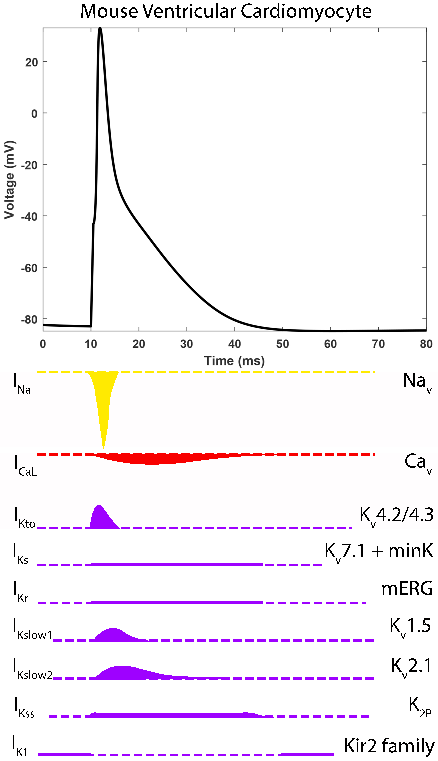
\includegraphics[scale=1]{figures/variety_currents.pdf}
    \caption{A schematic illustration of action potentials in mouse ventricular cardiomyocytes and underlying ionic currents of Na\textsubscript{v}, Ca\textsubscript{v}, and K\textsubscript{v} isoforms \cite{nerbonne2003molecular}.}
    \label{fig:variety_ionc}
\end{figure}

In contrast to Na\textsubscript{v} and Ca\textsubscript{v}, K\textsubscript{v} have a distinctive feature that they have multiple isoforms. Each isoform produces different but slightly overlapping component of the total K\textsuperscript{+} current (I\textsubscript{Ksum}) and contributes to different portions of the AP repolarization. To be specific, as shown in Figure~\ref{fig:variety_ionc}, there are various K\textsubscript{v} isoforms and currents they produce: the transient outward K\textsuperscript{+} current I\textsubscript{Kto} (K\textsubscript{v}4.2/K\textsubscript{v}4.3) several components of delayed rectifier K\textsuperscript{+} currents including I\textsubscript{Ks} (K\textsubscript{v}7.1 and minK), I\textsubscript{Kr} (mERG), I\textsubscript{Kslow1} (K\textsubscript{v}1.5), and I\textsubscript{Kslow2} (K\textsubscript{v}2.1), non-inactivating steady-state K\textsuperscript{+} current I\textsubscript{Kss} (K\textsubscript{2P}), and time independent K\textsuperscript{+} current I\textsubscript{K1} (Kir2 family) \cite{brouillette2004functional, liu2011dissection}. Note that although there are two types of transient outward currents, I\textsubscript{Ktof} and I\textsubscript{Ktos}, only one of them is presented and referred to as I\textsubscript{Kto} because I\textsubscript{Ktof} is only found in ventricular apex myocytes, while I\textsubscript{Ktos} is reported to appear only in the septum \cite{xu1999four}. There are several K\textsubscript{v} isoforms whose exact roles in shaping the cardiac AP are still subject of intensive research. Although it is highly desirable to study each unique K\textsuperscript{+} current rigorously, only I\textsubscript{Ksum} can be recorded during in-vitro experiments.

Hence, we need a data analysis tool to estimate individual K\textsuperscript{+} currents from I\textsubscript{Ksum}. Data assimilation is a scientific method that combines mathematical models and experimental data to calibrate the models; thereby, the in-silico models are compatible with the in-vitro observations. To be specific, for our case, a data assimilation method is required that couples mathematical models of K\textsuperscript{+} models with experimental data of I\textsubscript{Ksum} using whole-cell patch-clamp recordings to estimate various K\textsuperscript{+} currents. Exponential fitting is a traditional method based on the assumption that prominent K\textsuperscript{+} currents from patch-clamp recordings such as I\textsubscript{Kto}, I\textsubscript{Kslow1}, and I\textsubscript{Kslow2} have the shape of an exponential decay function $A_{i}e^{-t/\tau_{i}}$ as in Equation~\ref{eq:sumexp_model}, where $t$ is time variable, and $A_{i}$ and $\tau_{i}$ are the shape parameters. I\textsubscript{kss} is simplified as constant $A\textsubscript{Kss}$. It has been proven that exponential fitting accurately describes I\textsubscript{Ksum} with estimated K\textsuperscript{+} currents and has served as a standard method to analyze the sum of K\textsuperscript{+} currents \cite{brunet2004heterogeneous, liu2011dissection}. However, the mathematical model of this classical method only characterizes the shape of the currents, not the kinetics of corresponding K\textsubscript{v} isoforms. In addition, exponential fitting handles I\textsubscript{Ksum} recordings from the same cell with different conditions independently, so it lacks systematic analyses at the cellular level. 
\begin{equation}
    \text{I}\textsubscript{Ksum} = \sum_{i} A_{i} e^{-t/\tau_{i}} + A\textsubscript{Kss}, \; i \in I \subseteq \{\text{Kto, } \text{Kslow1, } \text{Kslow2}\} \label{eq:sumexp_model}
\end{equation}

On the other hand, computer models of cardiac electrophysiology can simulate complex dynamics of electrical activities at the cellular level that enable the quantitative understanding of biophysical functions such as gating kinetics of VGICs in the behavior of cardiomyocytes \cite{winslow2011integrative}. Therefore, this paper proposes a data assimilation method based on the computer models of K\textsubscript{v} isoforms that facilitates kinetics modeling at the cellular level. K\textsubscript{v} models are developed on biophysical principles of VGICs that are encoded in terms of mathematical equations. These equations have parameters that act like ``knobs'', allowing to control the behavior of the models. Tunning computer models to couple with experimental data requires trial-and-error investigations and domain knowledge in both the kinetics of cardiomyocytes and mathematics of computer models. Since modeling of cardiac electrophysiology is an interdisciplinary field that incorporates biology and engineering, calibration of computer models and interpretation of modeling results can be challenging for researchers in biology or medicine communities without engineering training. This hurdle hinders researchers in physiology from utilizing computer models to analyze their experimental data. A graphical user interface (GUI) is provided in which researchers can easily calibrate K\textsubscript{v} models to their data and visualize the modeling results. A new model calibration method will allow researchers to utilize computer models to analyze complex potassium dynamics in cardiomyocytes without engineering background. A GUI will provide an interactive environment to use the calibration method and analyze the results easily with visualizations.

\textbf{add a paragraph for case study with glycosylation and heart failure}

Cardiac electrophysiology has provided insights into the relationships between the complex dynamics of electrical signaling in the heart at the molecular level and the behavior of cardiomyocytes. Voltage-gated ion channels (VGICs) are the functional unit of electrical activities in cardiomyocytes. Among major cardiac VGICs, potassium channels have a distinctive feature in that they have multiple isoforms. Although each potassium isoform produces a unique current having different functionality, only the sum of these individual potassium currents (IKsum) can be recorded through in-vitro experiments. Hence there is an urgent need to develop a data analysis tool to estimate individual potassium currents from IKsum. Data assimilation is a scientific method that combines mathematical models and experimental data to calibrate the models; thereby, the in-silico models are compatible with the in-vitro observations. Exponential fitting is a traditional method based on the assumption that prominent potassium currents have the shape of an exponential decay function. However, the mathematical model of this classical method only characterizes the shape of the currents, not the kinetics of corresponding potassium channel isoforms. In addition, exponential fitting handles IKsum recordings from the same cell with different conditions independently, so it lacks systematic analyses at the cellular level. Therefore, this paper proposes a data assimilation method based on the computer models of potassium channel isoforms that facilitate kinetics modeling at the cellular level. A new data assimilation method is expected to allow researchers to estimate the kinetics of potassium isoforms from experimental IKsum data. 

% For Original Research articles, please note that the Material and Methods section can be placed in any of the following ways: before Results, before Discussion or after Discussion.

\section{Material and Methods}
\subsection{Procedure}
Least squares method \cite{reali2017optimization}.

\subsection{Data}

\section{Results}

\section{Conclusions}

\section{Formatting}

\subsection{Tables}
Tables should be inserted at the end of the manuscript. Please build your table directly in LaTeX.Tables provided as jpeg/tiff files will not be accepted. Please note that very large tables (covering several pages) cannot be included in the final PDF for reasons of space. These tables will be published as \href{http://home.frontiersin.org/about/author-guidelines#SupplementaryMaterial}{Supplementary Material} on the online article page at the time of acceptance. The author will be notified during the typesetting of the final article if this is the case. 

\section*{Conflict of Interest Statement}
%All financial, commercial or other relationships that might be perceived by the academic community as representing a potential conflict of interest must be disclosed. If no such relationship exists, authors will be asked to confirm the following statement: 

The authors declare that the research was conducted in the absence of any commercial or financial relationships that could be construed as a potential conflict of interest.

\section*{Author Contributions}

The Author Contributions section is mandatory for all articles, including articles by sole authors. If an appropriate statement is not provided on submission, a standard one will be inserted during the production process. The Author Contributions statement must describe the contributions of individual authors referred to by their initials and, in doing so, all authors agree to be accountable for the content of the work. Please see  \href{http://home.frontiersin.org/about/author-guidelines#AuthorandContributors}{here} for full authorship criteria.

\section*{Funding}
Details of all funding sources should be provided, including grant numbers if applicable. Please ensure to add all necessary funding information, as after publication this is no longer possible.

\section*{Acknowledgments}
This is a short text to acknowledge the contributions of specific colleagues, institutions, or agencies that aided the efforts of the authors.

\section*{Supplemental Data}
 \href{http://home.frontiersin.org/about/author-guidelines#SupplementaryMaterial}{Supplementary Material} should be uploaded separately on submission, if there are Supplementary Figures, please include the caption in the same file as the figure. LaTeX Supplementary Material templates can be found in the Frontiers LaTeX folder.

\section*{Data Availability Statement}
The datasets [GENERATED/ANALYZED] for this study can be found in the [NAME OF REPOSITORY] [LINK].
% Please see the availability of data guidelines for more information, at https://www.frontiersin.org/about/author-guidelines#AvailabilityofData

\bibliographystyle{frontiersinSCNS_ENG_HUMS} % for Science, Engineering and Humanities and Social Sciences articles, for Humanities and Social Sciences articles please include page numbers in the in-text citations
%\bibliographystyle{frontiersinHLTH&FPHY} % for Health, Physics and Mathematics articles
\bibliography{frontiers}

%%% Make sure to upload the bib file along with the tex file and PDF
\end{document}
